%% Copyright (C) 2009-2011, Gostai S.A.S.
%%
%% This software is provided "as is" without warranty of any kind,
%% either expressed or implied, including but not limited to the
%% implied warranties of fitness for a particular purpose.
%%
%% See the LICENSE file for more information.

\chapter{The UObject API}
\label{sec:uob:api}

The UObject API can be used to add new objects written in \Cxx to the
\us language, and to interact from \Cxx with the objects that are
already defined. We cover the use cases of controlling a physical
device (servomotor, speaker, camera\ldots), and interfacing
higher-lever components (voice recognition, object detection\ldots)
with \urbi.

The \Cxx API defines the UObject class. To each instance of a \Cxx class
deriving from UObject will correspond an \us object sharing some of its
methods and attributes. The API provides methods to declare which elements
of your object are to be shared. To share a variable with \urbi, you have to
give it the type UVar. This type is a container that provides conversion and
assignment operators for all types known to \urbi: \lstinline{double},
\lstinline{std::string} and \lstinline{char*}, and the binary-holding
structures \lstinline{UBinary}, \lstinline{USound} and
\lstinline{UImage}. This type can also read from and write to the liburbi
UValue class. The API provides methods to set up callbacks functions that
will be notified when a variable is modified or read from \urbi
code. Instance methods of any prototype can be rendered accessible from \us,
providing all the parameters types and the return type can be converted
to/from UValue.

\section{Compiling UObjects}

UObjects can be compiled easily directly with any regular compiler.
Nevertheless, \usdk provides two tools to compile UObject seamlessly.

In the following sections, we will try to compile a shared library named
\file{factory.so} (or \file{factory.dll} on Windows platforms) from a set of
four files (\file{factory.hh}, \file{factory.cc}, \file{ufactory.hh},
\file{ufactory.cc}).  These files are stored in a \file{factory.uob}
directory; its name bares no importance, yet the \file{*.uob} extension
makes clear that it is a UObject.

In what follows, \var{urbi-root} denotes the top-level directory of your
\usdk package, see \autoref{sec:install:install}.

\subsection{Compiling by hand}

On Unix platforms, compiling by hand into a shared library is
straightforward:

\begin{shell}
$ g++ -I \var{urbi-root}/include \
      -fPIC -shared \
      factory.uob/*cc -o factory.so
$ file factory.so
factory.so: ELF 32-bit LSB shared object, Intel 80386, \
  version 1 (SYSV), dynamically linked, not stripped
\end{shell}

On Mac OS X the flags \option{-Wl,-undefined,dynamic\_lookup} are needed:

\begin{shell}
$ g++ -I \var{urbi-root}/include \
      -shared -Wl,-undefined,dynamic_lookup \
      factory.uob/*.cc -o factory.so
$ file factory.so
factory.so: Mach-O 64-bit dynamically linked shared library x86_64
\end{shell}

\subsection{The \command{umake-*} family of tools}

\command{umake} can be used to compile UObjects.  See
\autoref{sec:tools:umake} for its documentation.

You can give it a list of files to compile:
\begin{shell}
$ umake -q --shared-library factory.uob/*.cc -o factory.so
umake: running to build library.
\end{shell}

\noindent
or directories in which \Cxx sources are looked for:

\begin{shell}
$ umake -q --shared-library factory.uob -o factory.so
umake: running to build library.
\end{shell}

\noindent
or finally, if you give no argument at all, the sources in the current
directory:

\begin{shell}
$ cd factory.uob
$ umake -q --shared-library -o factory.so
umake: running to build library.
\end{shell}


\subsection{Using the Visual \Cxx Wizard}

If you installed \usdk using its installer, and if you had Visual \Cxx
installed, then the UObject wizard was installed.  Use it to create your
UObject code:

\begin{center}
  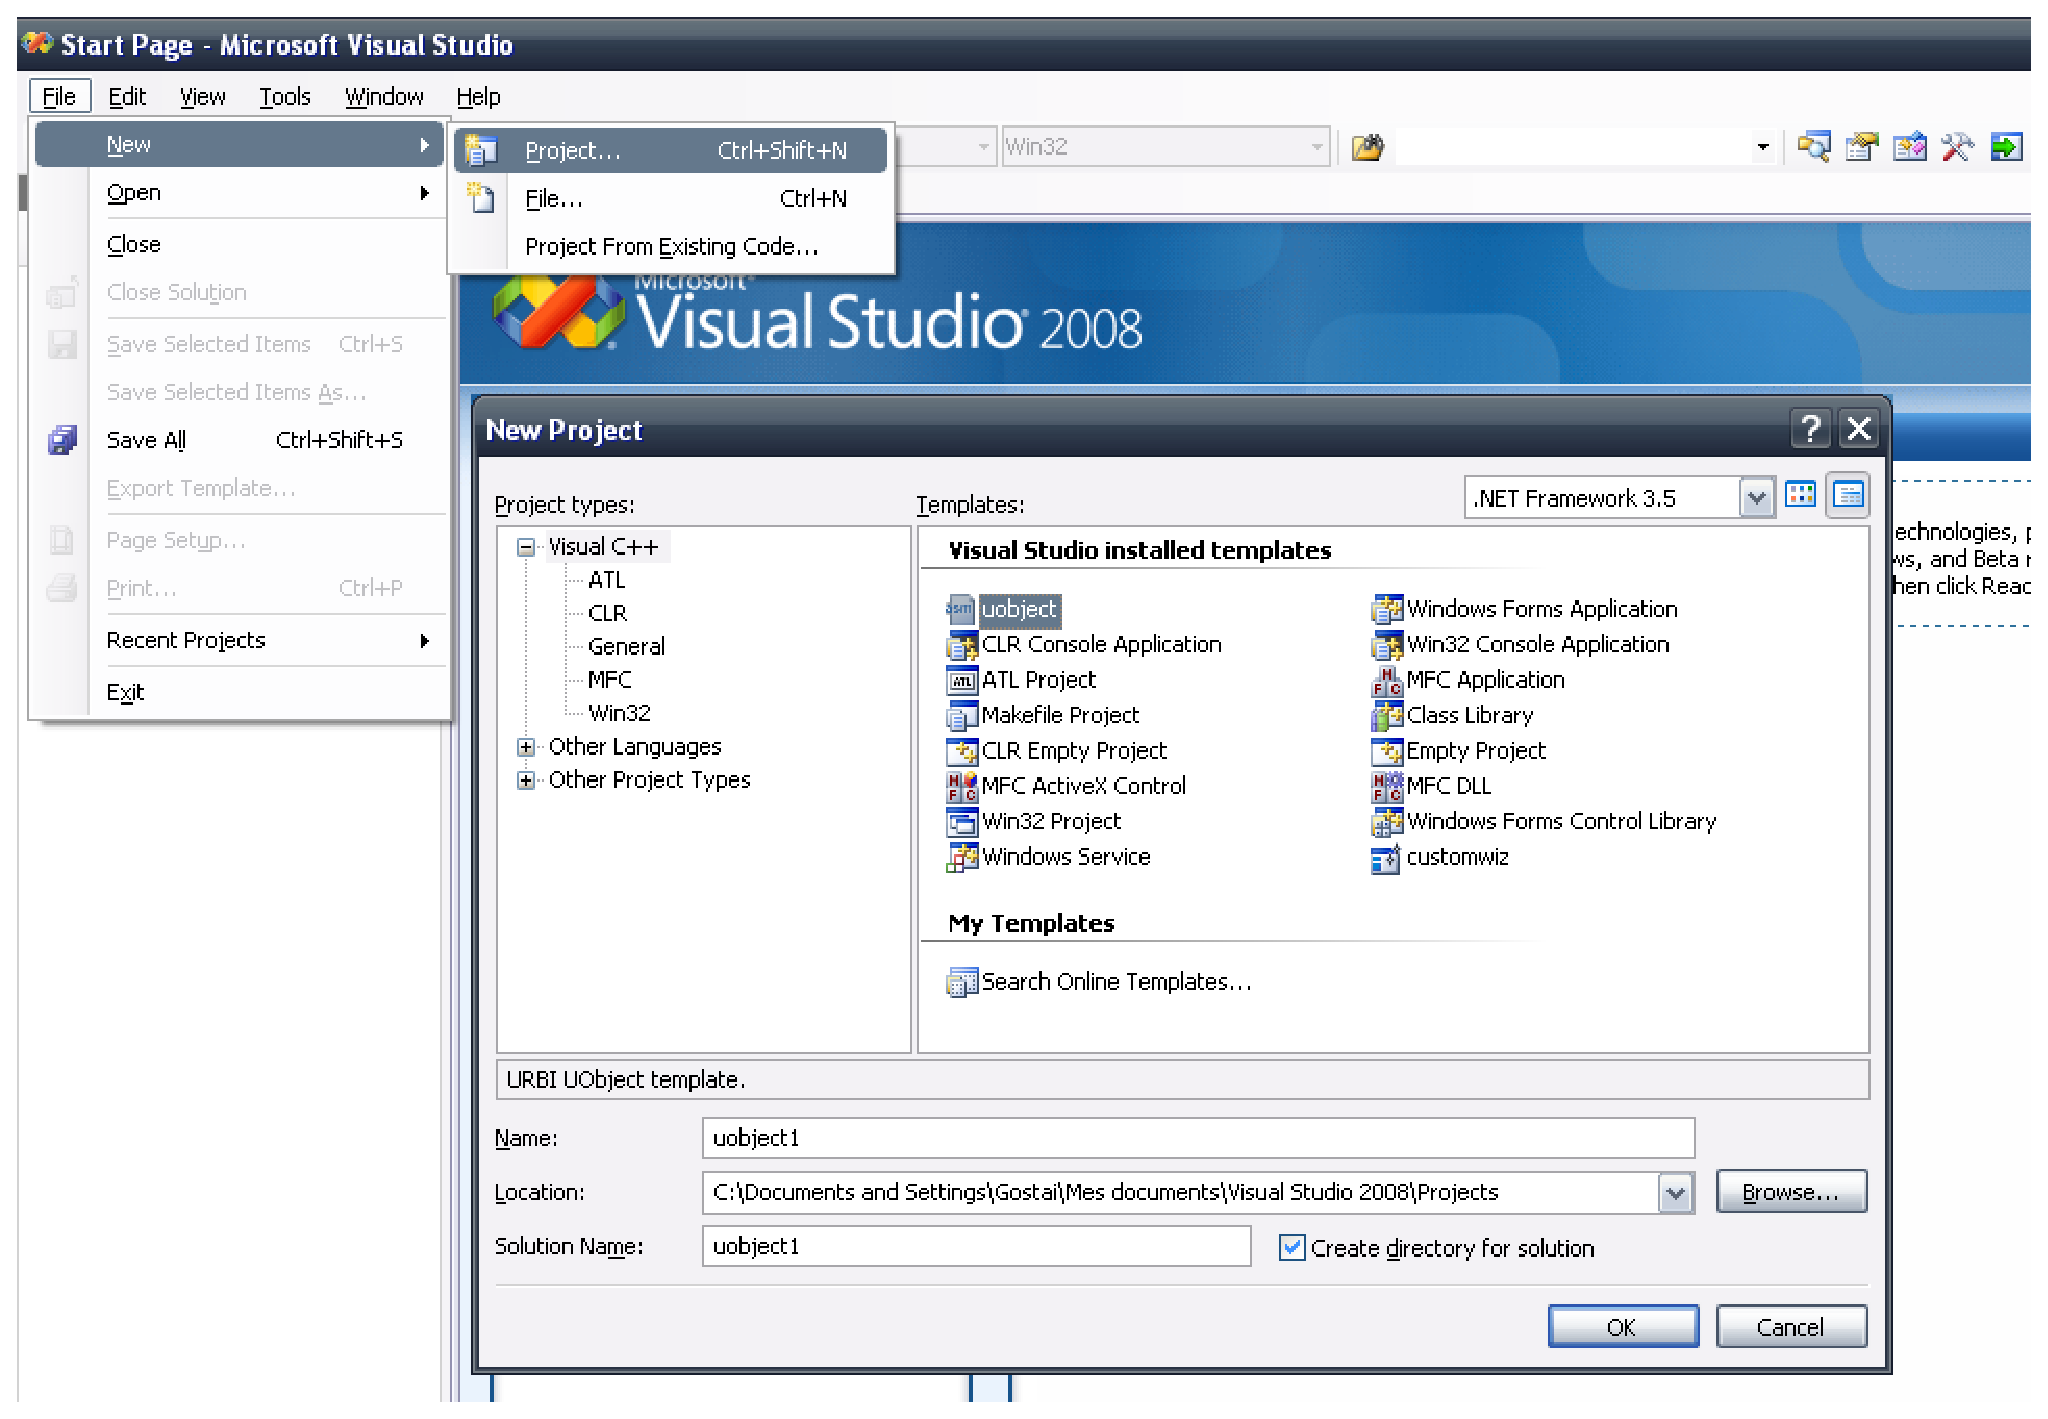
\includegraphics[width=0.6\linewidth]{img/visual-wizard-1}
\end{center}

Then, compile your UObject.

\begin{center}
  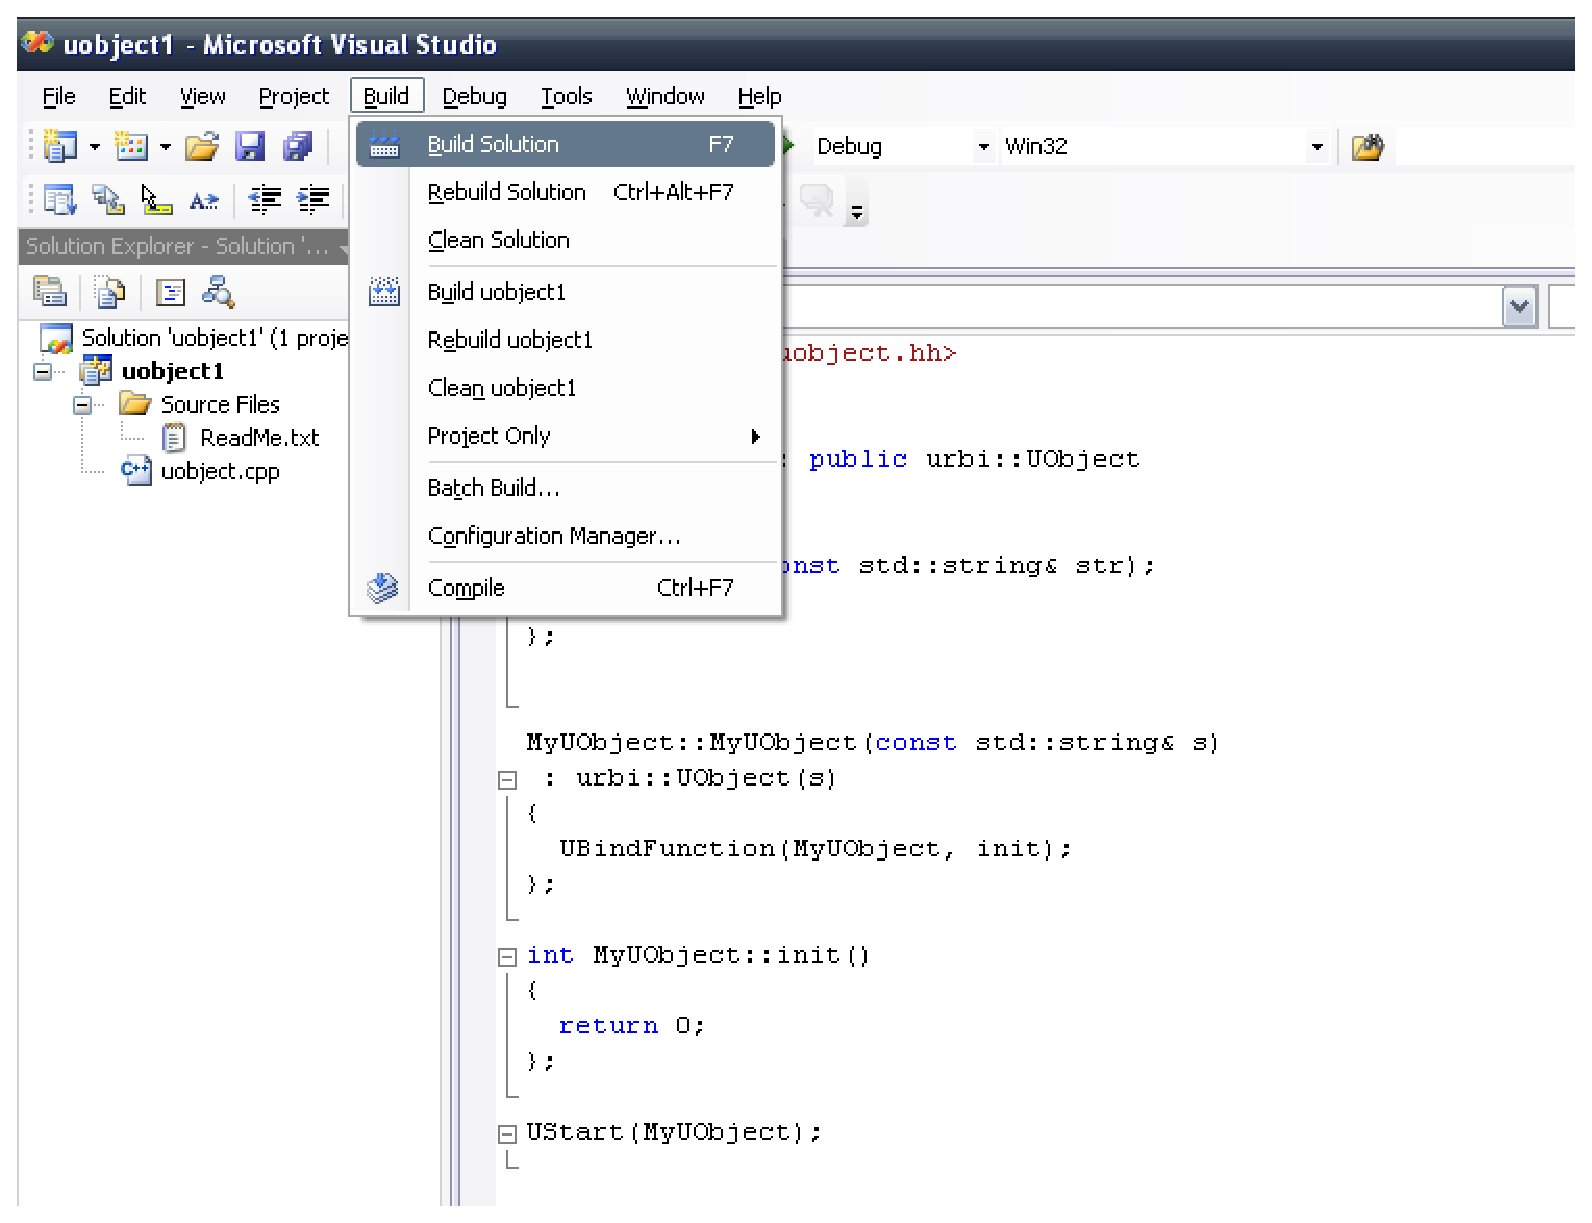
\includegraphics[width=0.6\linewidth]{img/visual-wizard-2}
\end{center}

And run it.

\begin{center}
  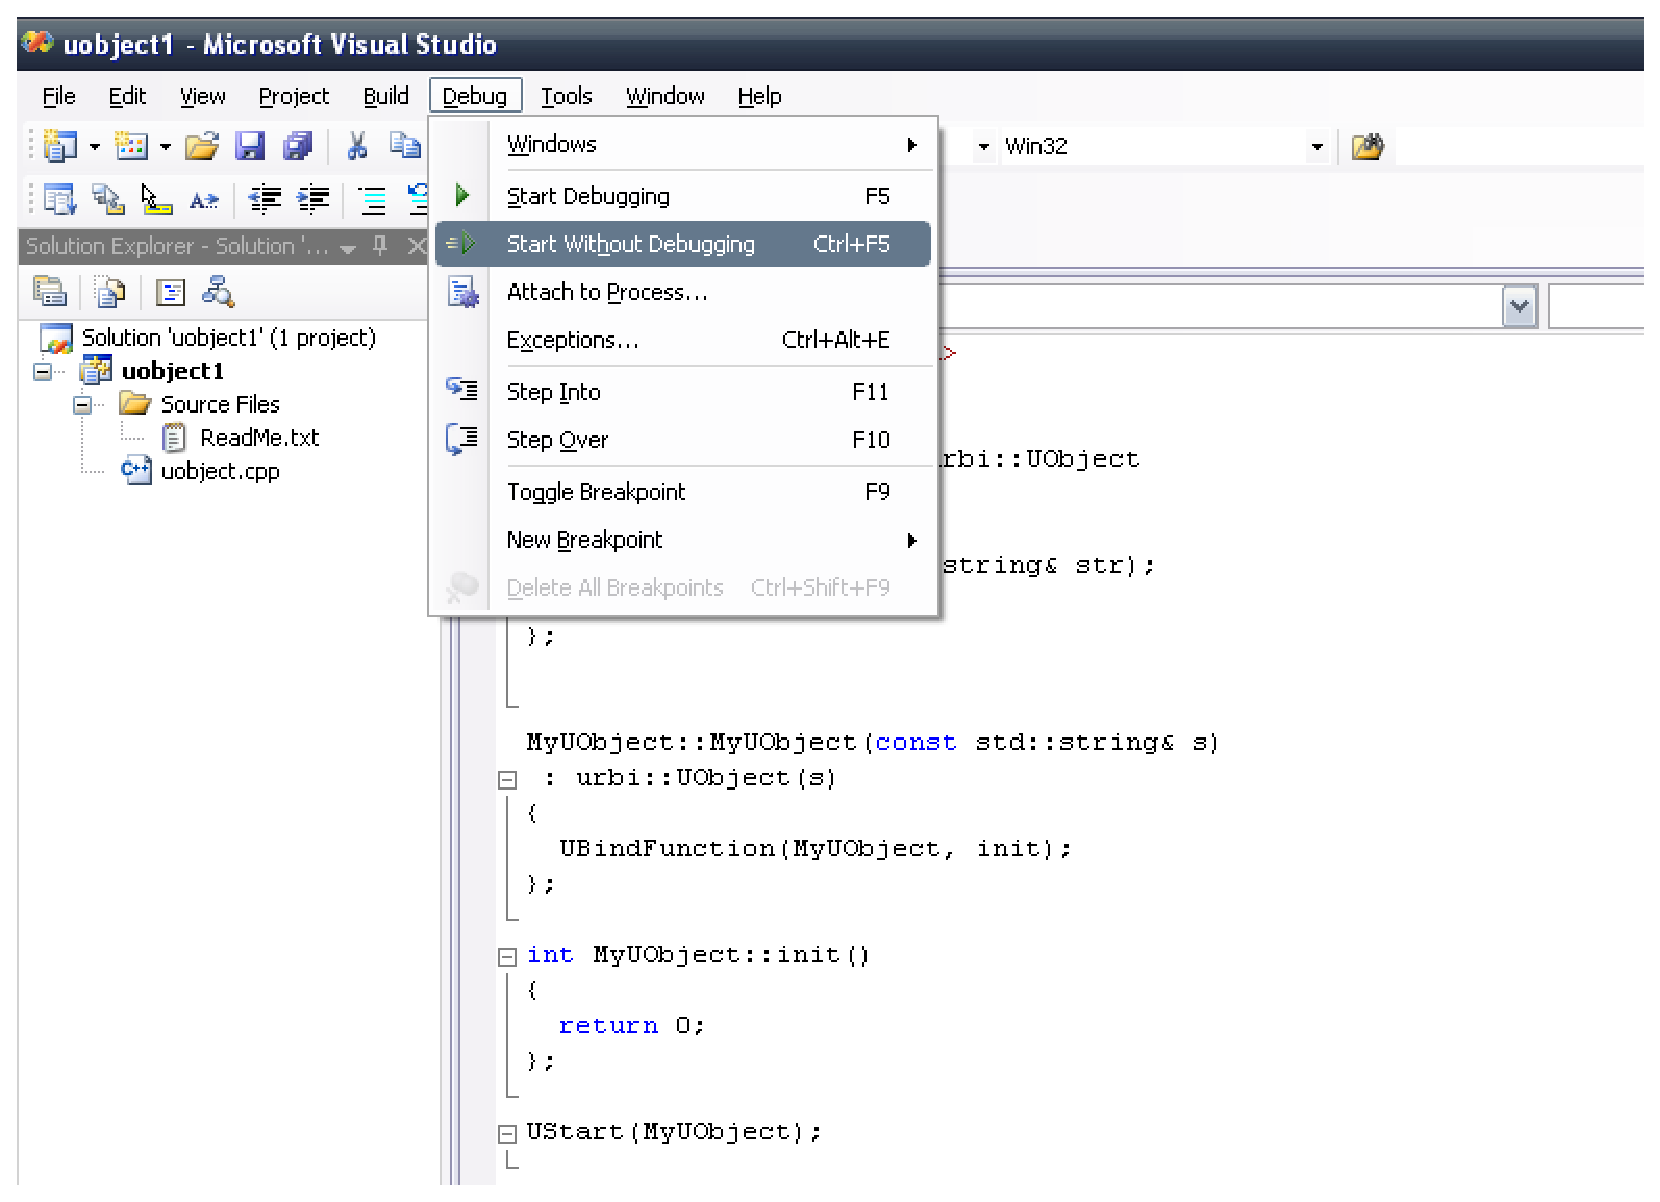
\includegraphics[width=0.6\linewidth]{img/visual-wizard-3}
\end{center}


\section{Creating a class, binding variables and functions}
\label{sec:uob:api:bind}

Let's illustrate those concepts by defining a simple object:
\lstinline{adder}. This object has one variable \lstinline{v}, and a method
\lstinline{add} that returns the sum of this variable and its argument.

\begin{itemize}
\item First the required include:

\begin{cxx}
#include <urbi/uobject.hh>
\end{cxx}

\item Then we declare our \lstinline{adder} class:
\begin{cxx}
class adder : public urbi::UObject // Must inherit from UObject.
{
  public:
   // The class must have a single constructor taking a string.
   adder(const std::string&);

   // Our variable.
   urbi::UVar v;

   // Our method.
   double add(double rhs) const;
};
\end{cxx}

\item The implementation of the constructor.
\begin{cxx}
// the constructor defines what is available from Urbi
adder::adder(const std::string& s)
  : urbi::UObject(s) // required
{
  // Bind the variable.
  UBindVar(adder, v);

  // Bind the function.
  UBindFunction(adder, add);
}
\end{cxx}

\item The implementation of our \lstinline{add} method.
\begin{cxx}
double
adder::add(double rhs) const
{
  return ((double) v) + rhs;
}
\end{cxx}
\item And register this class:
\begin{cxx}
// Register the class to the Urbi kernel.
UStart(adder);
\end{cxx}
\end{itemize}

To summarize:

\begin{itemize}
\item Declare your object class as inheriting from
  \lstinline{urbi::UObject}.
\item Declare a single constructor taking a string, and pass this
  string to the constructor of \lstinline{urbi::UObject}.
\item Declare the variables you want to share with \urbi with the type
  \lstinline{urbi::UVar}.
\item In the constructor, use the macros
  \lstinline|UBindVar(\var{class-name}, \var{variable-name})|
  for each \UVar you want as an instance variable, and
  \lstinline|UBindFunction(\var{class-name}, \var{function-name})| for
  each function you want to bind.
\item Call the macro \lstinline{UStart} for each object.
\end{itemize}

\section{Creating new instances}

When you start an \urbi server, an object of each class registered
with \lstinline{UStart} is created with the same name as the
class. New instances can be created from \urbi using the
\lstinline|new| method. For each instance created in \urbi, a
corresponding instance of the \Cxx object is created. You can get the
arguments passed to the constructor by defining and binding a method
named \lstinline|init| with the appropriate number of arguments.

\section{Binding functions}

\subsection{Simple binding}

You can register any member function of your \UObject using the macro

% Fix line wrap.
\lstinline|UBindFunction(\var{class-name}, \var{function-name})|.

Once done, the function can be called from \us.

The following types for arguments and return value are supported:

\begin{itemize}
\item Basic integer and floating types (int, double, float...).
\item \lstinline{const std::string&} or \lstinline{const char*}.
\item \lstinline{urbi::UValue} or any of its subtypes (\UBinary, \UList...).
\item \lstinline{std::list}, \lstinline{std::vector} or
\lstinline{boost::unordered_map} of the above types.
\end{itemize}

The procedure to register new types to this system is explained in
\autoref{sec:extend-cast-system}.

\subsection{Multiple bindings}
If you have multiple functions to bind, you can use the
\lstinline|UBindFunctions| macro to bind multiple functions at once:

\lstinline|UBindFunctions(\var{class-name}, \var{function1}, \var{function2}...)|.

\subsection{Asynchronous binding}
\label{sec:uobject:asynchronous-binding}
Functions bound using \lstinline{UBindFunction} are called synchronously, and
thus block everything until they return.

If you wish to bind a function that requires a non-negligible amount of time
to execute, you can have it execute in a separate thread by calling

% Separate line since lstinline does not word-wrap and this one is quite long.
\lstinline|UBindThreadedFunction(\var{class-name}, \var{function-name}, \var{lockMode})|.

The function code will be executed in a separate thread without breaking the
\us execution semantics.

The \var{lockMode} argument can be used to prevent parallel execution
of multiple bound functions if your code is not thread-safe. It can be any of
the following values.
\begin{itemize}
\item \lstinline{LOCK_NONE}\\
  No locking is performed.
\item \lstinline{LOCK_FUNCTION}\\
  Parallel execution is limited to one instance of the bound function.
\item \lstinline{LOCK_FUNCTION_DROP}\\
  Same as \lstinline{LOCK_FUNCTION}, but operations are dropped instead of
  being queued if one is already running.
\item \lstinline{LOCK_FUNCTION_KEEP_ONE}\\
  Same as \lstinline{LOCK_FUNCTION}, but the queue is limited to one, and
  subsequent calls are dropped.
\item \lstinline{LOCK_INSTANCE}\\
  Parallel execution is limited to one bound function for each object
  instance.
\item \lstinline{LOCK_CLASS}\\
  Parallel execution is limited to one bound function for the class.
\item \lstinline{LOCK_MODULE}\\
  Parallel execution is limited to one bound function for the whole module
  (shared object).
\end{itemize}

Other queue sizes can be used by passing
\lstinline{LockSpec(LOCK_FUNCTION, myQueueSize)} as \lstinline{lockMode}.

There is restriction to the locking mechanism: you cannot mix multiple locking
modes: for
instance a function bound with \lstinline{LOCK_FUNCTION} mode will not prevent
another function bound with \lstinline{LOCK_INSTANCE} from executing in
parallel.

You can perform your own locking using semaphores if your code needs a more
complex locking model.

You can limit the maximum number of threads that can run in parallel by using
the \lstinline{setThreadLimit} function.

\section{Notification of a variable change or access}
\label{sec:uobject:uvar-notify}
You can register a function that will be called each time a variable is
modified by calling \lstinline{UNotifyChange(var, func)}.

\begin{itemize}
\item \lstinline{var} must be either the name of an \UVar, or an \UVar itself.
\item \lstinline{func} must be a member function of your \UObject. This function
will be called each time the \UVar receives a new value.
\end{itemize}

The function can take 0 or 1 argument. If the argument is of type
\lstinline{UVar&}, then the function will receive the \UVar that was passed to
\lstinline{UNotifyChange}. If it is of any other type, then the new value in the
\UVar will be converted to this type and passed to the function.

In plugin mode, there is a similar mechanism to create a {\em getter function}
that will be called each time an \UVar is accessed: the
\lstinline{UNotifyAccess} function. It has the same signature as
\lstinline{UNotifyChange}, and calls the given function each time someone tries
to access the \UVar. The function can update the value in the \UVar before
the access takes place. Usage of \lstinline{UNotifyAccess} should be reserved
to infrequently used \UVar that take a long time to update, as it disrupts
the data flow between \UObject.


You can remove all notifies associated to any given \UVar by calling its
\lstinline{unnotify} function.


\section{Data-flow based programming: exchanging UVars}

The \lstinline{UNotifyChange} and \lstinline{UNotifyAccess} features
can be used to link multiple UObjects together, and perform data-flow
based programming: the \lstinline{UNotifyChange} can be called to
monitor UVars from other UObjects.  Those UVars can be transmitted
through bound function calls.

One possible pattern is to have each data-processing UObject take its
input from monitored UVars, given in its constructor, and output the
result of its processing in other UVars. Consider the following
example of an object-tracker:

\begin{cxx}
class ObjectTracker: public urbi::UObject
{
public:
  ObjectTracker(const std::string& n)
    : urbi::UObject(n)
  {
    // Bind our constructor.
    UBindFunction(ObjectTracker, init);
  }
  // Take our data source in our constructor.
  void init(UVar& image)
  {
    UNotifyChange(image, &ObjectTracker::onImage);
    // Bind our output variable.
    UBindVar(ObjectTracker, val);
  }
  void onImage(UVar& src)
  {
    UBinary b = src;
    // Processing here.
    val = processing_result;
  }
  UVar val;
};
UStart(ObjectTracker);
\end{cxx}

The following \us code would be used to initialize an ObjectTracker given a
camera:

\begin{urbiunchecked}
var tracker = ObjectTracker.new(camera.&val);
\end{urbiunchecked}

An other component could then take the tracker output as its input.

Using this model, chains of processing elements can be created. Each time the
UObject at the start of the chain updates, all the notifyChange will be called
synchronously in cascade to update the state of the intermediate components.

\section{Data-flow based programming: InputPort}
\label{sec:uob:input-port}

\urbi provides a second and more standard way to perform data-flow
programming.  In this approach, inputs of a component are declared as local
InputPort, and the binding between this InputPort and the output of another
component is done in \us using the \lstinline|>>| operator between two
\UVar:

\begin{cxx}
class ObjectTracker: public urbi::UObject
{
  ObjectTracker(const std::string& n)
    : urbi::UObject(n)
  {
    // Bind our constructor.
    UBindFunction(ObjectTracker, init);
    // Bind our input port.
    UBindVar(ObjectTracker, input);
    // NotifyChange on our own input port
    UNotifyChange(input, &ObjectTracker::onImage);
  }
  // Init is empty
  void init()
  {
  }
  // onImage is unchanged.
  void onImage(UVar& src)
  {
    UBinary b = src;
    // Processing here.
    val = processing_result;
  }
  UVar val;
  // Declare our input port.
  InputPort input;
};
UStart(ObjectTracker);
\end{cxx}

In this model, linking the components is done in \us:

\begin{urbiunchecked}
var tracker = ObjectTracker.new();
camera.&val >> tracker.&input;
\end{urbiunchecked}

\subsection{Customizing data-flow links}
\defObject{UConnection}
The \lstinline|>>| operator to establish a data-flow link between two \UVar
returns an object of type \refObject{UConnection} that can be used to customize
the link.

This object is also present in the slot \lstinline|changeConnections| of the
source \UVar.

Here is the list of \dfn{UConnection} slots:

\begin{urbiscriptapi}
\item[enabled]
  Set to false to disable the link.
\item[minInterval]
  Minimal interval in seconds at which the link can activate. Changes of the
  source at a higher rate will be ignored.
\item[asynchronous]
  If true, notifies on the target InputPort will trigger asynchronously. The
  system will also prevent two instances from running in parallel by dropping
  updates until the callback functions terminate.
\item[disconnect]
  Disconnect the link.
\item[reconnect](<src>)
  Reconnect the link by changing the source to \var{src}.
\item[callCount]
  Number of times the link was reset.
\item[fireRate]
  Rate in Hertz at which the link triggers.
\item[meanCallTime]
  Average time taken by the callback function on the target InputPort.
\item[minCallTime]
  Minimum call time.
\item[maxCallTime]
  Maximum call time.
\item[resetStats]
  Reset all statistics.
\item[getAll]
  Return the list of all the connections in the system.
\end{urbiscriptapi}


The function \lstinline|uobjects.connectionStats()| can be used to display
the statistics of all the connections, and
\lstinline|uobjects.resetConnectionStats()| can be called to reset all
statistics.

\section{Timers}
\label{sec:uob:timers}

The API provides two methods to have a function called periodically:
\begin{cxxapi}
\item[void urbi::UObject::USetUpdate(ufloat period)] Set up a timer that
  calls the virtual method \lstinline{UObject::update()} with the specified
  period (in milliseconds).  Disable updates if \var{period} is -1.

\item[urbi::TimerHandle urbi::UObject::USetTimer<T>(ufloat period, void (T::*fun)())]
  Invoke an UObject member function \var{fun} every \var{period}
  milliseconds.  \var{fun} is a regular member-function pointer, for
  instance \lstinline|MyUObject::my_function|.
  The function returns a \lstinline|TimerHandle| that can be passed to the
  \lstinline|UObject::removeTimer(h)| function to disable the timer.
\end{cxxapi}

\section{The special case of sensor/effector variables}

In \urbi, a variable can have a different meaning depending on whether you
are reading or writing it: you can use the same variable to represent the
target value of an effector and the current value measured by an associated
sensor. This special mode is activated by the \UObject defining the variable
by calling \lstinline{UOwned} after calling \lstinline{UBindVar}. This call
has the following effects:
\begin{itemize}
\item When \urbi code or code in other modules read the variable, they read
  the current value.
\item When \urbi code or code in other modules write the variable, they set
  the target value.
\item When the module that called \lstinline|UOwned| reads the variable, it
  reads the target value. When it writes the variable, it writes the current
  value.
\end{itemize}

\section{Using \urbi variables}

The C++ class \UVar is used to represent any \urbi slot in C++.  To bind the
\UVar to a specific slot, pass its name to the \UVar constructor, or its
\lstinline|init| method.  Once the \UVar is bound, you can write any
compatible type to it, and the new value will be visible in \us.  Similarly,
you can cast the \UVar (or use the \lstinline{as()} method) to convert the
current \us value held to any compatible type.

Compatible types are the same as for bound functions (see
\autoref{sec:extend-cast-system}).

\begin{cxx}
// Set the camera format to 0 if it is 1.
UVar v;
v.init("camera", "format");
if (v == 1)
 v = 0;
\end{cxx}

Some care must be taken in remote mode: changes on the variable coming from
\urbi code or an other module can take time to propagate to the \UVar. By
default, all changes to the value will be sent to the remote \UObject. To
have more control on the bandwidth used, you can disable the automatic
update by calling \lstinline|unnotify()|. Then you can get the value on
demand by calling \lstinline|UVar::syncValue()|.

\begin{cxx}
UVar v("Global", "x");
send("every|(100ms) Global.x = time,");
// At this point, v is updated approximately every 100 milliseconds.

v.unnotify();
// At this point v is no longer updated. If v was the only UVar pointing to
// 'Global.x', the value is no longer transmitted.

v.syncValue();
// The previous call will ask for the value of Global.x once, and block until
// the value is written to v.
\end{cxx}

You can read and write all the \urbi properties of an \UVar by
reading and writing the appropriate \lstinline{UProp} object in the
\UVar.

\section{Emitting events}

The \UEvent class can be used to create and emit \us events. Instances are
created and initialized exactly as \UVar: either by using the
\lstinline{UBindEvent} macro, or by calling one of its constructors or the
\lstinline{init} function.

Once initialized, the \lstinline{emit} function will trigger the emission of
the associated \us event. It can be called with any number of arguments, of
any compatible type.

\section{UObject and Threads}

The \UObject API is thread-safe in both plugin and remote mode: All API
calls including operations on \UVar can be performed from any thread.

\section{Using binary types}

\urbi can store binary objects of any type in a generic container, and
provides specific structures for sound and images. The generic containers is
called \UBinary and is defined in the \file{urbi/ubinary.hh} header. It
contains an enum field type giving the type of the binary
(\lstinline{UNKNOWN}, \lstinline{SOUND} or \lstinline{IMAGE}), and an union
of a \USound and \UImage struct containing a pointer to the data, the size
of the data and type-specific meta-information.

\subsection{UVar conversion and memory management}
The \UBinary manages its memory: when destroyed (or going out-of-scope), it
frees all its allocated data. The \USound and \UImage do not.

Reading an \UBinary from a \UVar, and writing a \UBinary, \USound or \UImage
to an \UVar performs a deep-copy of the data (by default, see below).

Reading a \USound or \UImage from an \UVar performs a shallow
copy. Modifying the data is not allowed in that case.

\subsection{0-copy mode}
In plugin mode, you can setup any \UVar in 0-copy mode by calling
\lstinline{setBypass(true)}. In this mode, binary data written to the \UVar
is not copied, but a reference is kept.  As a consequence, the data is only
available from within registered notifyChange callbacks. Those callbacks can
use \lstinline|UVar::val()| or cast the \UVar to a \UBinary\& to retrieve
the reference.  Attempts to read the \UVar from outside notifyChange will
result in \lstinline{nil} being returned.

\section{Using hubs to group objects}

Sometimes, you need to perform actions for a group of \lstinline{UObjects},
for instance devices that need to be updated together. The API provides the
\UObjectHub class for this purpose. To create a hub, simply declare a
subclass of \UObjectHub, and register it by calling once the macro
\lstinline|UStartHub (\var{class-name})|. A single instance of this class
will then be created upon server start-up. \UObject instances can then
register to this hub by calling %
\lstinline|URegister (\var{hub-class-name})|. %
Timers can be attached to \UObjectHub the same way as to \UObject (see
\autoref{sec:uob:timers}). The kernel will call the \lstinline{update()}
method of all \UObject before calling the \lstinline{update()} method of the
hub. A hub instance can be retrieved by calling
\lstinline{getUObjectHub (string classname)}. The hub also holds the list of
registered UObject in its members attribute.

\section{Sending \us code}

If you need to send \us code to the server, the \lstinline{URBI()}
macro is available, as well as the \lstinline{send()} function. You
can either pass it a string, or directly \urbi code inside a double
pair of parentheses:

\begin{urbiunchecked}
send ("myTag:1+1;");

URBI (( at (myEvent?(var x)) { myTag:echo x; }; ));
\end{urbiunchecked}

You can also use the \lstinline{call} method to make an urbiscript function
call:

\begin{urbiunchecked}
// C++ equivalent of urbiscript 'System.someFunc(12, "foo");'
call("System", "someFunc", 12, "foo");
\end{urbiunchecked}

\section{Using RTP transport in remote mode}
\label{sec:uob:api:rtp}

By default, \urbi uses TCP connections for all communications between the
engine and remote UObjects. \urbi also supports the UDP-based \dfn{RTP}
protocol for more efficient transmission of updated variable values. RTP
will provide a lower latency at the cost of possible packet loss, especially
in bad wireless network conditions.

\subsection{Enabling RTP}

To enable RTP connections, both the engine and the remote-mode urbi-launch
containing your remote \UObject must load the RTP \UObject. This can be
achieved by passing \lstinline|urbi/rtp| as an extra argument to both
urbi-launch command lines (one for the engine, the other for your remote
\UObject).

Once done, all binary data transfer (like sound and image) in both
directions will by default use a RTP connection.

\subsection{Per-UVar control of RTP mode}

You can control whether a specific \UVar uses RTP mode by calling its
\lstinline|useRTP(bool)| function. Each binary-type \UVar will have its own
RTP connection, and all non-binary \UVar will share one.

From \us, you can also write to the \lstinline|rtp| slot of each UVar. Existing
notifies will be modified to use rtp if you set it to true.


\section{Extending the cast system}
\label{sec:extend-cast-system}

\subsection{Principle}

The same cast system is used both for bound function's arguments and return
values, and for reading/writing \UVar.

Should you want to add new type \lstinline{MyType} to the system you must define
two functions:

\begin{cxx}
namespace urbi
{
  void operator, (UValue& v, const MyType& t)
  { // Here you must fill v with the serialized representation of t.
  }
  template<> struct uvalue_caster<MyType>
  {
    MyType operator()(UValue& v)
    { // Here you must return a MyType made with the information in v.
    }
  }
}
\end{cxx}

Once done, you will be able without any other change to
\begin{itemize}
\item Take MyType as argument to a bound function.
\item Return a MyType from a bound function.
\item Write a MyType to an \UVar.
\item Convert an \UVar to MyType using the \lstinline{UVar::as} function.
\end{itemize}

\subsection{Casting simple structures}

The system provides facilities to serialize simple structures by value between
C++ and \us. This system uses two declarations of each structure, one in
C++ and the other in \urbi, and maps between the two.

Here is a complete commented example to map a simple Point structure between
\us and C++.
\begin{cxx}
struct Point
{
  // Your struct must have a default constructor.
  Point():x(0), y(0) {}
  double x,y;
};

// Declare the structure to the cast system. First argument is the struct,
// following arguments are the field names.
URBI_REGISTER_STRUCT(Point, x, y);
\end{cxx}

\begin{urbiunchecked}
// Declare the urbiscript structure. It must be globally accessible, and
// inheriting from UValueSerializable.
class Global.Point: UValueSerializable
{
  var x = 0;
  var y = 0;
  function init(xx=0, yy=0)
  {
     x = xx|
     y = yy
  };
  function asString()
  {
    "<" + x +", " + y  + ">"
  };
};
// Add the class to Serializables to register it.
var Serializables.Point = Point;
\end{urbiunchecked}

Once done, you can call bound functions taking a C++ Point by passing them
an \us Point and exchange Point between both worlds through \UVar read/write.

%%% Local Variables:
%%% mode: latex
%%% TeX-master: "../urbi-sdk"
%%% ispell-dictionary: "american"
%%% ispell-personal-dictionary: "../urbi.dict"
%%% fill-column: 76
%%% End:
